\documentclass[italian,usepdftitle=false]{beamer}
\usetheme{dmpisa}

\usepackage[T1]{fontenc}
\usepackage[utf8]{inputenc}
\usepackage[italian]{babel}
\usepackage{amsmath,amssymb}
\usepackage{mathpazo}
\usepackage{array,booktabs,multirow,tabularx}
\usepackage{tikz}
\usetikzlibrary{arrows.meta,calc,positioning}

\usefonttheme[onlymath]{serif}
\titlebackground*{assets/background}

\AtBeginSection[]{}
\makeatletter
\patchcmd{\beamer@checkframetitle}
  {\framesubtitle{\thesection \, \secname}}{}{}{}
\makeatother

\newcommand{\NN}{\mathbb{N}}
\newcommand{\RR}{\mathbb{R}}
\newcommand{\RE}{\mathrm{RE}}
\newcommand{\RecTot}{\mathsf{Rec}_{\mathrm{tot}}}
\DeclareMathOperator{\ev}{ev}
\DeclareMathOperator{\Hom}{Hom}
\definecolor{lawverered}{RGB}{225,78,72}
\definecolor{lawveregreen}{RGB}{45,205,140}

\setbeamertemplate{theorem begin}{%
  \begin{\inserttheoremblockenv}{%
    \rmfamily\bfseries\inserttheoremname%
    \ifblank{\inserttheoremaddition}{}{ (\inserttheoremaddition)}%
  }%
  \rmfamily
}
\setbeamertemplate{theorem end}{\end{\inserttheoremblockenv}}

\setbeamertemplate{proof begin}{%
  \begin{block}{\rmfamily\bfseries\insertproofname}%
  \rmfamily
}
\setbeamertemplate{proof end}{\end{block}}

\setbeamertemplate{itemize item}{\color{maincolor}\small$\blacktriangleright$}
\setbeamertemplate{itemize subitem}{\color{maincolor}\scriptsize$\bullet$}
\setlength{\tabcolsep}{5pt}
\newcolumntype{L}[1]{>{\raggedright\arraybackslash}p{#1}}
\newcolumntype{Y}{>{\raggedright\arraybackslash}X}

\tikzset{
  flow/.style={-{Latex[length=2.2mm]},line width=1.1pt,draw=maincolor},
  flowgray/.style={-{Latex[length=2.2mm]},line width=1pt,draw=darkgray},
  concept/.style={rounded corners=3pt,draw=maincolor,line width=.9pt,
    fill=sintefgrey,align=center,inner sep=6pt},
  accent/.style={rounded corners=3pt,draw=sintefgreen,line width=1pt,
    fill=sinteflightgreen,align=center,inner sep=6pt},
  logicaccent/.style={rounded corners=3pt,draw=sinteflilla,line width=1pt,
    fill=sinteflilla!8,align=center,inner sep=6pt},
  categoryaccent/.style={rounded corners=3pt,draw=maincolor,line width=1pt,
    fill=maincolor!8,align=center,inner sep=6pt},
  flowaccent/.style={-{Latex[length=2.2mm]},line width=1.1pt,draw=sintefgreen},
  warning/.style={rounded corners=3pt,draw=sintefred,line width=1pt,
    fill=sintefred!8,align=center,inner sep=6pt}
}

\title{Lawvere's Fixed-Point Theorem through the Curry--Howard--Lambek Correspondence}
\subtitle{Relatore: Prof.\ Marcello Mamino}
\course{Corso di Laurea Triennale in Matematica\\Università di Pisa}
\author{Diego Monaco}
\date{25 settembre 2026}

\begin{document}
\maketitle

\section{Punti fissi e diagonalizzazione}

\begin{frame}{Teoremi di punto fisso}
  \small
  \centering
  \begin{tikzpicture}[node distance=5mm and 5mm]
    \node[concept,text width=30mm,font=\bfseries] (fixed) {Teoremi di punto fisso};
    \node[warning,below left=of fixed,text width=40mm] (general)
      {Geometrici, topologici\\e di ordinamenti};
    \node[accent,below right=of fixed,text width=40mm] (diagonal)
      {Diagonali: formalizzano\\l'autoreferenzialità};
    \draw[flow] (fixed) -- (general);
    \draw[flow] (fixed) -- (diagonal);
    \node[below=4mm of general,align=center,font=\footnotesize] (examples_left)
      {Brouwer \quad Banach \quad Tarski\\ punti fissi di operatori normali\\ \ldots};
    \draw[flow] (general) -- (examples_left);
    \node[below=4mm of diagonal,align=center,font=\footnotesize] (examples)
      {Cantor \quad Russell \quad Gödel\\Turing \quad Rogers \\ \ldots};
    \draw[flow] (diagonal) -- (examples);
  \end{tikzpicture}
\end{frame}

\begin{frame}{Punto fisso nel caso diagonale}
  \centering
  \vspace*{2mm}
  \begin{tikzpicture}
    \node[rounded corners=3pt,draw=maincolor,line width=1pt,fill=white,
          text width=108mm,align=left,inner sep=7pt,font=\small]
      {Tipicamente, nei casi diagonali, si ha una mappa $\phi:A\times A\to B$, detta \textcolor{maincolor}{\textbf{codifica universale}} (o semplicemente codifica), che codifica ogni mappa $d : A \to B$,
      i.e., esiste un codice $a_d$ per cui $\phi(a_d,-)=d(-)$.\\[1mm]};
  \end{tikzpicture}

  \vspace{2mm}
  \uncover<2->{Presa $f : B \to B$ possiamo allora:}\par
  \vspace{2mm}
  \begin{tikzpicture}[node distance=7mm]
    \uncover<2->{
    \node[accent,text width=32mm,minimum height=21mm] (diag)
      {\textbf{1. Diagonalizzare}\\[3pt]
       $d(x):=f\bigl(\phi(x,x)\bigr)$};}
    \only<3->{
    \node[accent,right=of diag,text width=32mm,minimum height=21mm] (code)
      {\textbf{2. \mbox{Prenderne} il codice}\\[3pt]
       $\phi(p,-)=d(-)$};}
    \only<4->{
    \node[accent,right=of code,text width=32mm,minimum height=21mm] (self)
      {\textbf{3. Applicare la funzione al codice}\\[3pt]
       $s:=\phi(p,p)$};}
    \only<3->{\draw[flowaccent] (diag) -- (code);}
    \only<4->{\draw[flowaccent] (code) -- (self);}
  \end{tikzpicture}

  \vspace{-2mm}
  \uncover<5>{
  \[
    s=\phi(p,p)=d(p)=f\bigl(\phi(p,p)\bigr)=f(s)
  \]
  }
\end{frame}

\section{Il teorema di Lawvere}

\begin{frame}{Dove formalizzare il principio diagonale}
  \small
  \vspace{1mm}
  \makebox[\linewidth][c]{\parbox{\dimexpr\linewidth+4mm\relax}{Il setting per formalizzare il principio diagonale è quello delle categorie cartesiane/cartesiane chiuse.}}

  \vspace{1mm}
  \begin{block}{\textbf{Categoria cartesiana}}
    Una \textbf{categoria cartesiana} è una categoria con prodotti finiti, ossia:
    \begin{itemize}
      \item un oggetto terminale $1$;
      \item prodotti binari $A\times B$ per ogni coppia di oggetti $A,B$.
    \end{itemize}
  \end{block}

  \vspace{3mm}
  \begin{block}{\textbf{Categoria cartesiana chiusa}}
    Una \textbf{categoria cartesiana chiusa} è una categoria cartesiana che ammette:
    \begin{itemize}
      \item un esponenziale $B^A$ per ogni coppia di oggetti $A,B$, con la
        proprietà di indurre una bigezione:
        \[
          \Hom(X\times A,B)\cong\Hom(X,B^A).
        \]
    \end{itemize}
  \end{block}
\end{frame}

\begin{frame}<1-2>[t]{Lawvere formalizza il principio diagonale}
  \small
  Lawvere generalizza il principio precedente: una codifica universale forza
  punti fissi.

  \vspace{0mm}
  \begin{block}{Teorema di Lawvere (1969)}
    \vspace{1mm}
    \begin{columns}[T,onlytextwidth]
      \begin{column}{.47\textwidth}
        \centering
        \textcolor{maincolor}{\textbf{Forma esponenziale}}\par\smallskip
        In una categoria cartesiana chiusa, se\par\smallskip
        $\phi:A\longrightarrow B^A$\par\smallskip
        è debolmente suriettiva sui punti,
      \end{column}
      \begin{column}{.47\textwidth}
        \centering
        \textcolor{maincolor}{\textbf{Forma diagonale}}\par\smallskip
        In una categoria cartesiana, se\par\smallskip
        $\Phi:A\times A\longrightarrow B$\par\smallskip
        è debolmente suriettiva sui punti,
      \end{column}
    \end{columns}

    \vspace{2mm}
    \centering
    {\color{darkgray}\rule{.82\linewidth}{.4pt}}\par\smallskip
    \textbf{allora}:
    ogni endomorfismo $f:B\to B$ ammette un punto fisso
    $s:1\to B$, cioè $f\circ s=s$.
  \end{block}

  \uncover<2->{%
  \vspace{1mm}
  \centering
  In una categoria cartesiana chiusa le due forme sono equivalenti per currying:
  \[
    \phi=\Phi^*
    \quad\Longleftrightarrow\quad
    \Phi=\phi^\sharp,
  \]
  \vspace{-3mm}
  dove\;
  \((-)^*\colon\!\Hom(A\times A,B)
    \overset{\cong}{\to}\Hom(A,B^A), \quad
    (-)^\sharp\colon\!\Hom(A,B^A)
    \overset{\cong}{\to}\Hom(A\times A,B).\)
  \vspace{-1mm}
  }
\end{frame}

\section{Curry--Howard--Lambek}
\vspace{1mm}
\begin{frame}{Curry--Howard--Lambek}
  \framesubtitle{Il trinitarismo computazionale}
  \centering
  \vspace{3mm}
  \begin{tikzpicture}[node distance=15mm]
    \node[logicaccent,text width=32mm,minimum height=18mm] (logic)
      {\textbf{Logica intuizionista}\\proposizioni\\dimostrazioni};
    \node[accent,right=of logic,text width=32mm,minimum height=18mm] (lambda)
      {\textbf{$\lambda$-calcolo tipato}\\tipi\\programmi};
    \node[categoryaccent,right=of lambda,text width=32mm,minimum height=18mm] (cat)
      {\textbf{Categorie}\\\textbf{cartesiane chiuse}\\oggetti / morfismi};
    \draw[flowgray] ([yshift=2mm]logic.east)
      -- node[midway,above=1mm,font=\tiny,fill=white,inner sep=.5pt]
         {Curry--Howard}
      ([yshift=2mm]lambda.west);
    \draw[flowgray] ([yshift=-2mm]lambda.west)
      -- node[midway,below=1mm,inner sep=0pt]
         {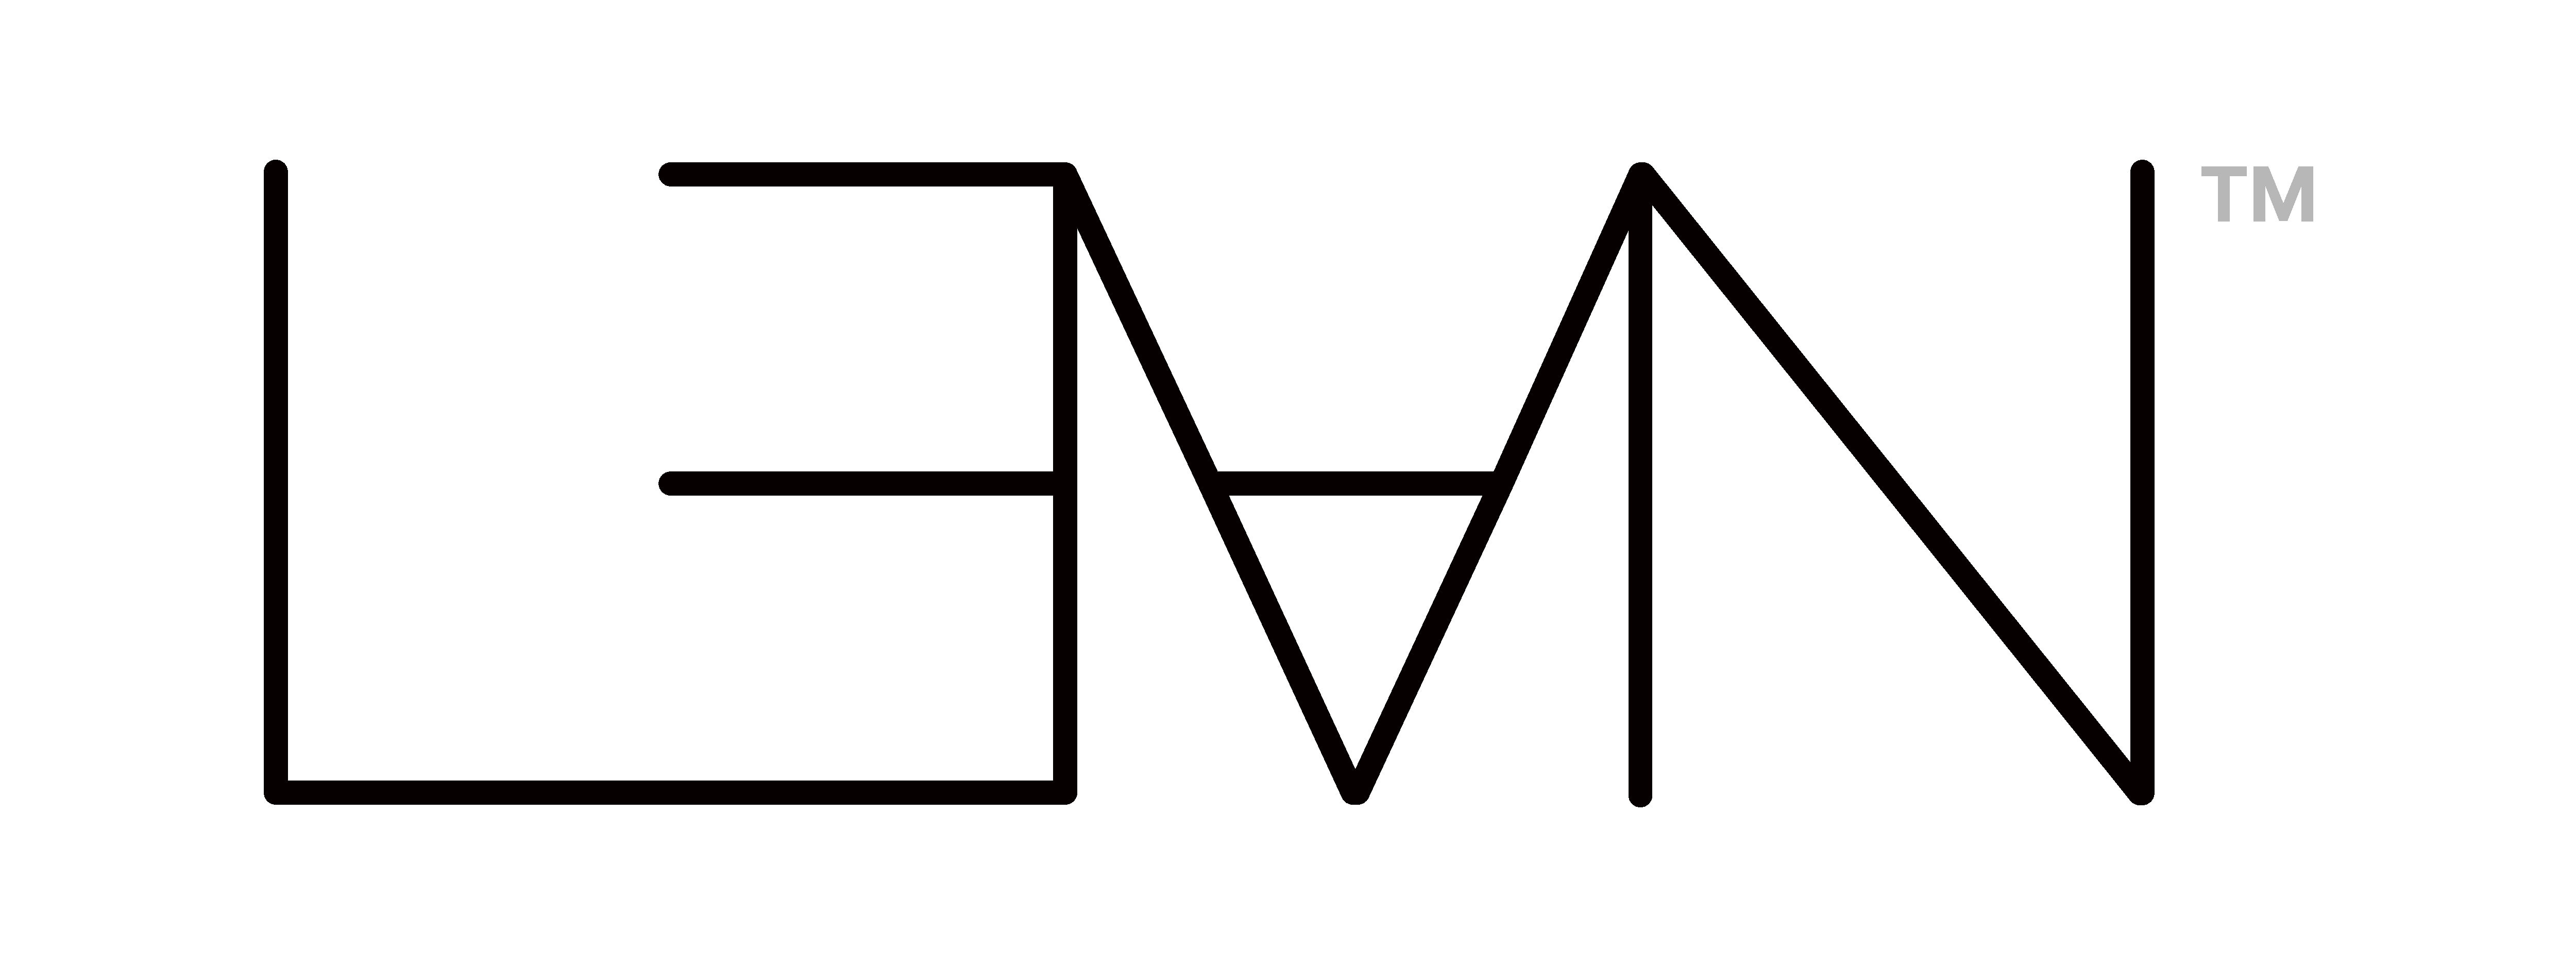
\includegraphics[width=7mm]{../images/lean-logo-official-TM-transparent.pdf}}
      ([yshift=-2mm]logic.east);
    \draw[flowgray] ([yshift=2mm]lambda.east)
      -- node[midway,above=1mm,font=\tiny,fill=white,inner sep=.5pt]
         {Lambek}
      ([yshift=2mm]cat.west);
    \draw[flowgray] ([yshift=-2mm]cat.west) -- ([yshift=-2mm]lambda.east);
  \end{tikzpicture}

  \vspace{3mm}
  \begin{block}{Equivalenza di categorie}
    \centering
    $\mathsf{CCC}_N \simeq \lambda\text{-}\mathsf{Calc}_N$

    \vspace{-1mm}
    \footnotesize
    \renewcommand{\arraystretch}{.9}
    \begin{tabularx}{.97\textwidth}{@{}p{15mm} >{\raggedright\arraybackslash}X c p{15mm} >{\raggedright\arraybackslash}X@{}}
      \multicolumn{2}{c}{\color{maincolor}\bfseries $\mathsf{CCC}_N$}
        & &
      \multicolumn{2}{c}{\color{sintefgreen}\bfseries $\lambda\text{-}\mathsf{Calc}_N$} \\[-1.4mm]
      \multicolumn{2}{c}{\color{maincolor}\rule{42mm}{.7pt}}
        & &
      \multicolumn{2}{c}{\color{sintefgreen}\rule{42mm}{.7pt}} \\[-.2mm]
      \smash{{\color{maincolor}\bfseries oggetti}}
        & CCC con WNNO e iteratore
        & {\color{darkgray}\normalsize $\longleftrightarrow$}
        & \smash{{\color{sintefgreen}\bfseries oggetti}}
        & $\lambda$-calcoli tipati \\[.6mm]
      \smash{{\color{maincolor}\bfseries morfismi}}
        & funtori che preservano la \mbox{struttura} cartesiana chiusa
        & {\color{darkgray}\normalsize $\longleftrightarrow$}
        & \smash{{\color{sintefgreen}\bfseries morfismi}}
        & traduzioni tra calcoli tipati
    \end{tabularx}
  \end{block}
  \hfill{\scriptsize Lambek--Scott, 1986}
\end{frame}

\section{Applicazioni di Lawvere}

\begin{frame}{Applicazioni di Lawvere}
  \centering
  Il teorema di Lawvere ci permette di ottenere due famiglie di risultati.\par
  \vspace{2mm}
  \begin{columns}[T,onlytextwidth]
    \begin{column}{.47\textwidth}
      {\setbeamercolor{block title}{fg=black,bg=lawveregreen}
      \setbeamercolor{block body}{fg=black,bg=lawveregreen!25}
      \begin{block}{Teoremi di esistenza}
        Se esiste un morfismo "surgettivo" $\phi$ dello stesso tipo,
        allora ogni endomorfismo $f:B\to B$ ammette un punto fisso:
        \[
          \exists s : 1 \to B \qquad f \circ s = s.
        \]
      \end{block}
      }
    \end{column}
    \begin{column}{.47\textwidth}
      {\setbeamercolor{block title}{fg=black,bg=lawverered}
      \setbeamercolor{block body}{fg=black,bg=lawverered!25}
      \begin{block}{Teoremi di impossibilità}
        Se un oggetto $B$ ammette un endomorfismo senza punti fissi, allora non esiste una mappa "surgettiva" del tipo:
        \[
          \phi : A \times A \to B \quad\text{ o }\quad \phi : A \to B^A.
        \]
      \end{block}
      }
    \end{column}
  \end{columns}

  \vspace{3mm}
  \begin{center}
    \begin{minipage}{\textwidth}
      \centering\normalsize\color{darkgray}
      Vediamo alcuni esempi concreti in
      \textbf{teoria degli insiemi, topologia, calcolabilità e logica}.
    \end{minipage}
  \end{center}
\end{frame}

\begin{frame}{Applicazioni di Lawvere}
  \framesubtitle{Teoria degli insiemi e topologia}
  \scriptsize
  \renewcommand{\arraystretch}{1.30}
  \setlength{\tabcolsep}{4pt}
  \begin{tabularx}{\textwidth}{@{}>{\centering\arraybackslash}p{.09\textwidth} >{\bfseries}L{.14\textwidth} L{.24\textwidth} Y@{}}
    \toprule
    \textcolor{maincolor}{\bfseries Categoria}
      & Risultato & Mappa senza punti fissi & Cosa non può essere universale \\
    \midrule
    \multirow{3}{*}[-6mm]{\textcolor{maincolor}{$\mathsf{Set}$}}
      & Cantor
      & $\neg : \{0,1\} = 2 \to 2$
      & Nessuna suriezione $A\twoheadrightarrow2^A$; in particolare, adattando la dimostrazione di Lawvere nel caso di $\NN$ e $\RR$,
      si ottiene l'argomento diagonale di Cantor, per cui $|\NN|<|\RR|$.\\
    & Russell
      & ancora $\neg:2\to2$
      & Se la classe $V$ fosse un insieme, $a\mapsto\mathbf1_a$ darebbe
        $V\twoheadrightarrow2^V$: impossibile. \\
    & Paradossi classici
      & negazione su $2$ o permutazione su $3$
      & Barbiere, Grelling e mentitore (forte) si basano tutti sul fatto che non esiste una mappa $\phi : A \times A \twoheadrightarrow \{0,1\}$,
      perché altrimenti codificherebbe la mappa $a \mapsto \neg\phi(a,a)$. \\
    \addlinespace[.7mm]
    \textcolor{maincolor}{$k\mathsf{Top}$}
      & Suriezioni continue
      & un $t:X\to X$ continuo senza punti fissi
      & Nessuna suriezione continua $I\twoheadrightarrow X^I$;
        ad esempio: $S^1$ con la mappa antipodale, gruppi topologici non banali, lo spazio di Cantor $2^{\NN}$. \\
    \bottomrule
  \end{tabularx}
\end{frame}

\begin{frame}{Applicazioni di Lawvere}
  \framesubtitle{Teoria della calcolabilità}
  \scriptsize
  \renewcommand{\arraystretch}{1.30}
  \setlength{\tabcolsep}{4pt}
  \begin{tabularx}{\textwidth}{@{}>{\centering\arraybackslash}p{.13\textwidth} >{\bfseries}L{.18\textwidth} Y L{.215\textwidth}@{}}
    \toprule
    \textcolor{maincolor}{\bfseries Categoria}
      & Risultato & Enunciato & Significato \\
    \midrule
    \multirow{3}{*}[-15mm]{\textcolor{maincolor}{$\mathsf{Asm}(\mathcal K_1)$}}
      & Teorema di Rice
      & Se $R\subseteq\NN$ è estensionale e decidibile, allora
        $R=\varnothing$ oppure $R=\NN$.
      & Una proprietà estensionale non banale non è decidibile. \\
    & Teorema di punto fisso per operatori estensionali
      & Se $F:\RE\to\RE$ è estensionale, allora esiste $n\in\NN$ tale che
        $F(W_n)=W_n$.
      & Ogni operatore estensionale sugli insiemi r.e. ammette un punto fisso. \\
    & Teorema di Rogers
      & Se $\varphi:\NN\to\NN$ è ricorsiva totale, allora esiste $n\in\NN$
        con $u_1(\varphi(n),-)=u_1(n,-)$.
      & Ogni funzione ricorsiva totale manda il codice di almeno un programma in un altro codice di un programma equivalente. \\
    \addlinespace[.7mm]
    \textcolor{maincolor}{$\mathcal C$ (CCC)}
      & Oggetti riflessivi
      & Se $U$ è riflessivo, esiste $Y:U^U\to U$ con
        $\ev_{U,U}\circ\langle 1_{U^U},Y\rangle=Y$.
      & $Y$ sceglie uniformemente un punto fisso per ogni endomorfismo di $U$. \\
    \bottomrule
  \end{tabularx}
\end{frame}

\begin{frame}{Applicazioni di Lawvere}
  \framesubtitle{Ancora calcolabilità: enumerazioni uniformi e linguaggi}
  \scriptsize
  \renewcommand{\arraystretch}{.85}
  \setlength{\tabcolsep}{3pt}
  \makebox[\textwidth][c]{\begin{tabularx}{\dimexpr\textwidth+12mm\relax}{@{}>{\centering\arraybackslash}p{.10\textwidth} >{\bfseries}L{.19\textwidth} Y L{.27\textwidth}@{}}
    \toprule
    \textcolor{maincolor}{\bfseries Categoria}
      & Risultato & Enunciato & Significato \\
    \midrule
    \multirow{5}{*}[-15mm]{\textcolor{maincolor}{$\RecTot$}}
      & Halting problem
      & L'halting set $H_1 = \{ (\alpha, x) \in \NN^2 | u_1(\alpha, x) \ne \bot \}$ non è decidibile.
      & Non esiste un algoritmo che decide se un programma termina. \\
    & Enumerazione funzioni ricorsive totali
      & Detta $(f_n)_{n\in\NN}$ un'enumerazione delle funzioni ricorsive totali, non esiste $F(-,-)$ ricorsiva totale
      tale che $F(n,-)=f_n$ per ogni $n\in\NN$.
      & Non esiste un algoritmo che elenchi tutti e soli i programmi che terminano su ogni input. \\
    & Enumerazione insiemi decidibili
      & Detta $(A_n)_{n\in\NN}$ un'enumerazione degli insiemi decidibili, non esiste $G(-,-)$ ricorsiva totale
      tale che $A_n = \{G(n,-) = 0\}$.
      & Non esiste un algoritmo che elenchi tutti gli insiemi decidibili. \\
    & Insiemi semidecidibili
      & Esiste un insieme semidecidibile $A\subseteq\NN$ con complementare $A^{\complement}$ non semidecidibile.
      & Saper semi-decidere un insieme non significa saper semidecidere il suo complementare. \\
    & Insieme delle verità aritmetiche
      & $\mathrm{Th}(\NN;L_{\textnormal{arit}})$ non è ricorsivamente enumerabile.
      & Non c'è un algoritmo che riconosce tutte le proposizioni aritmetiche vere in $\NN$. \\
    \addlinespace[.2mm]
    \textcolor{maincolor}{$\mathsf{Set}$}
      & Esistenza di un linguaggio non r.e.
      & Esiste un linguaggio $L\subseteq\{1\}^*$ non r.e.
      & Esiste un linguaggio le cui stringhe non possono essere riconosciute da un algoritmo. \\
    \bottomrule
  \end{tabularx}}
\end{frame}

\begin{frame}<1-4>{Vediamo un esempio in dettaglio}
  \framesubtitle{L'halting problem in $\RecTot$}
  \small
  \begin{block}{Halting problem (Turing, 1937)}
    \centering
    L'halting set $H_1 = \{ (\alpha, x) \in \NN^2 | u_1(\alpha, x) \ne \bot \}$ non è decidibile.
  \end{block}

  \vspace{2mm}
  \centering
  \uncover<2->{%
  \begin{tikzpicture}[node distance=5mm,
      haltingstep/.style={text width=128mm,inner xsep=4pt,inner ysep=3pt,font=\small}]
    \node[categoryaccent,haltingstep] (total)
      {\mbox{$F(e,x)=\begin{cases}
         \text{output del programma }e\text{ su }x & \text{se termina}\\
         0 & \text{altrimenti}
       \end{cases}$}};

    \uncover<3->{
      \node[accent,haltingstep,below=of total] (universal)
        {Per ogni funzione calcolabile totale $g : \NN \to \NN$, esiste un suo \textit{codice} $\ulcorner g \urcorner$ tale che\\[2pt]
         \mbox{$F(\ulcorner g \urcorner,x)=g(x)\quad\forall x\in\NN$}.};
      \draw[flow] (total) -- (universal);
    }

    \uncover<4->{
      \node[warning,haltingstep,below=of universal] (contradiction)
        {\mbox{Quindi ogni funzione calcolabile totale $\NN\to\NN$ avrebbe un punto fisso, ma}\\[2pt]
         \mbox{$s:\NN\to\NN:n\mapsto n+1$}\\[2pt]
         {\settowidth{\dimen0}{Quindi ogni funzione calcolabile totale $\NN\to\NN$ avrebbe un punto fisso, ma}%
          \makebox[\dimen0][l]{non ha punti fissi, assurdo.}}};
      \draw[flow] (universal) -- (contradiction);
    }
  \end{tikzpicture}
  }
\end{frame}

\begin{frame}{Primo teorema di incompletezza di Gödel}
  \small
  \begin{block}{Teorema di incompletezza (Gödel, 1931)}
    \centering
    Se $T$ è una teoria aritmetica coerente e ricorsivamente assiomatizzabile,\\
    con $\mathsf{PA}\subseteq T$ e $\NN\models T$, allora $T$ è incompleta.
  \end{block}

  \vspace{2mm}
  \centering
  \begin{tikzpicture}[
      x=1mm,y=1mm,
      endpoint/.style={rounded corners=3pt,draw=maincolor,line width=1pt,
        fill=maincolor,text=white,align=center,inner sep=5pt},
      semanticroute/.style={rounded corners=3pt,draw=sinteflilla,line width=1pt,
        fill=sinteflilla!8,align=center,inner sep=5pt},
      syntacticroute/.style={rounded corners=3pt,draw=sintefgreen,line width=1pt,
        fill=sinteflightgreen!55,align=center,inner sep=5pt},
      semanticflow/.style={flow,draw=sinteflilla},
      syntacticflow/.style={flow,draw=sintefgreen}
    ]
    \node[endpoint,text width=23mm,minimum height=19mm,font=\bfseries]
      (lawvere) at (-4,0)
      {Teorema di Lawvere\\[.4mm]};
    \node[semanticroute,text width=56mm,minimum height=13mm,font=\bfseries]
      (satisfaction) at (51.5,-11.5)
      {$\mathsf{Sat}$ non è definibile in $T$\\[.4mm]
       {\scriptsize\mdseries\spaceskip=0pt\xspaceskip=0pt Lawvere in $\mathsf{Lind}_T$}};
    \node[syntacticroute,text width=56mm,minimum height=19mm,font=\bfseries]
      (diagonal) at (51.5,11.5)
      {Lemma di diagonalizzazione di Gödel\\[.4mm]
       {\scriptsize\mdseries\spaceskip=0pt\xspaceskip=0pt Adattando la dimostrazione di Lawvere in $\mathsf{Set}$}};
    \node[endpoint,text width=23mm,minimum height=19mm,font=\bfseries]
      (godel) at (107,0)
      {Gödel\\[.4mm]
       {\scriptsize\mdseries\spaceskip=0pt\xspaceskip=0pt Incompletezza di $T$}};

    \draw[semanticflow] ([yshift=-3mm]lawvere.east) -- (satisfaction.west);
    \draw[semanticflow] (satisfaction.east) -- ([yshift=-3mm]godel.west);
    \draw[syntacticflow] ([yshift=3mm]lawvere.east) -- (diagonal.west);
    \draw[syntacticflow] (diagonal.east) -- ([yshift=3mm]godel.west);
  \end{tikzpicture}
\end{frame}

\section{McCallum e Brouwer}

\begin{frame}{Per Brouwer, Lawvere classico non basta}
  \small
  \begin{block}{Teorema (Brouwer, 1911)}
    \raggedright
    Sia $D$ una palla chiusa in uno spazio euclideo di dimensione finita. Si ha che ogni mappa continua $f:D\to D$ ha un punto fisso, cioè esiste $x\in D$ tale che $f(x)=x$.
  \end{block}

  \vspace{0mm}
  \raggedright
  L'applicazione diretta di Lawvere richiede una suriezione continua, che non esiste nemmeno in un caso molto semplice come:
  {\setlength{\abovedisplayskip}{2pt}
  \setlength{\abovedisplayshortskip}{2pt}
  \setlength{\belowdisplayskip}{2pt}
  \setlength{\belowdisplayshortskip}{2pt}
  \[
    A\twoheadrightarrow[0,1]^A.
  \]}
  \vspace{-3mm}
  \begin{colorblock}[white]{sintefred}{Ostacolo (McCallum, 2020)}
    In $\mathsf{ZFC}$ non esiste alcuno spazio topologico $A$ per cui sia
    definita la topologia esponenziale su $[0,1]^A$ ed esista una suriezione continua $A\twoheadrightarrow[0,1]^A$.
  \end{colorblock}

  \vspace{2mm}
  {\centering
    \begin{tikzpicture}[node distance=8mm,scale=.9,transform shape]
      \node[concept] (law) {Lawvere classico};
      \node[warning,dashed,right=of law] (missing) {ipotesi topologica\\non realizzabile};
      \node[concept,right=of missing] (brouwer) {Brouwer};
      \draw[flow] (law) -- (missing);
      \draw[flow] (missing) --
        node[midway,inner sep=0pt,text=sintefred,font=\LARGE] {$\boldsymbol{\times}$}
        (brouwer);
    \end{tikzpicture}
  \par}
\end{frame}

\begin{frame}{Idea: usare due topologie diverse}
  \small
  \raggedright
  Equipaggiando lo stesso insieme $|A|$ con una topologia più fine $\tau'$ e una
  meno fine $\tau''$, allora possono esistere mappe continue e surgettive:
  \[
    A' := (|A|,\tau') \twoheadrightarrow X^{(|A|,\tau'')} =: X^{A''}.
  \]

  \vspace{-2.1mm}
  \begin{block}{Lawvere generalizzato (McCallum, 2020)}
    \footnotesize
    Siano $\mathcal C$ una categoria cartesiana, $\mathcal S$ una sua sottoclasse, $A',A'' \in \mathcal C$ e $h:A'\to A''$ puntualmente bigettiva.
    Se per ogni $X\in\mathcal S$ esiste $g_X:A'\to X^{A''}$ puntualmente surgettiva e se ogni $q:A'\to X$, che fattorizza
    attraverso $\langle g_X,h\rangle$, fattorizza anche attraverso $h$, allora
    ogni endomorfismo degli oggetti di $\mathcal S$ ha un punto fisso.
  \end{block}

  \vspace{-2.1mm}
  {\setbeamercolor{block title}{fg=white,bg=sintefgreen}
  \setbeamercolor{block body}{fg=darkgray,bg=sintefgrey}
  \begin{block}{Proposizione (McCallum, 2020)}
    \footnotesize
    Esiste una opportuna sottoclasse di spazi $\mathcal S\subseteq k\mathsf{Top}$, contenente tutte le
    palle chiuse degli spazi euclidei di dimensione finita, tale che per ogni $X\in\mathcal S$ le ipotesi del teorema precedente sono soddisfatte.
  \end{block}
  }
\end{frame}

\begingroup
  \themecolor{main}
  \begin{frame}[c]
    \centering
    \usebeamercolor[fg]{normal text}
    {\Huge\textsl{Grazie per l'attenzione!}}
  \end{frame}
\endgroup

\end{document}
